\documentclass[11pt]{article}

\usepackage{kotex}
\usepackage{sectsty}
\usepackage{graphicx}
\usepackage{amsmath}

% Margins
\topmargin=-0.45in
\evensidemargin=0in
\oddsidemargin=0in
\textwidth=6.5in
\textheight=9.0in
\headsep=0.25in


\title{ Vi }
\author{asdasdㅁㅁㅁㅁㅇ가나다 MinWook Kang }
\date{\today}

\begin{document}
\maketitle
\pagebreak

% Optional TOC
% \tableofcontents
% \pagebreak

%--Paper--

\section{Section 1}
\noindent
dsdasdfasd
\begin{equation}
    f(x) = y \lambda
\end{equation}

\begin{figure}[!ht]
  \centering
  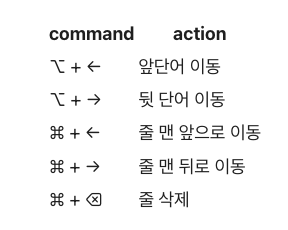
\includegraphics[width=0.5\textwidth]{mac.png}
  \caption{Bessel Function}
\end{figure}

\pagebreak
\section{Section 2}
Lorem Ipsum \\

%--/Paper--

\end{document}
